\section{Development, Implementation, and Testing}
\subsection{Environment and PI Controller}
Training a neural network to act as a load frequency controller using DDPG requires a simulated model of a two area power system. This will be referred to as the environment model. The environment model developed by this research will consist of two power areas connected via a tie-line, each with a governor, turbine, and generator. The model will take 2 control action inputs --- one for each power system area. The model will be designed to output 7 values including governor states, turbine states, and power system frequencies for each area, in addition to the power transfer of the tie-line.

The mathematical representation of the environment model will be developed in the temporal domain. This design choice is motivated by the need to stop and start the simulation periodically, allowing the neural network to take simulation states as inputs, and issue control action outputs. Upon receiving a control action the simulation will iterate forward by some discrete time interval, using previous stopping states as initial conditions. This could not be achieved in the frequency domain as initial conditions are assumed to be zero. The temporal domain model will be developed by taking inverse Laplace transforms of frequency domain models from simulation experiments discussed in the literature review.

A PI controller model will be developed to provide a performance benchmark comparison for the neural network. The model will take 3 inputs from the environment model, namely the frequency from each power system area, and the tie-line power transfer. Whilst the PI controller could be developed in the frequency domain, for convenience it will be developed in the temporal domain to interact with the temporal environment model of the two area power system. The PI controller model will be mathematically specified using the same methodology described for the two area power system environment model.

Model parameter values for the two area power system model will be selected based on a review of the most common model parameters observed in the literature review. Tuned model parameters for the PI controller will selected to ensure near optimal control performance.

\subsection{Neural Network and DDPG Algorithm}
Neural network actor-critic models will be designed to have an input layer, 2 hidden layers, and an output layer. This design choice was motivated by Lillicrap \textit{et alias} \cite{Lillicrap2015}. The input layer will be designed to receive 7 model inputs, consisting of governor and turbine states for each power system area, frequencies for each power system area, and the power transfer on the tie-line. The output layer will issue 2 control actions to be received by the environment model.

The neural network model will be developed to allow for modification to the number of nodes and activation functions in hidden layers. This design choice has been made to facilitate investigation of neural network control performance with respect to model architecture changes based on the work by Henderson \textit{et alias} \cite{Henderson2017}.

The DDPG algorithm will be developed based on Algorithm \ref{alg:ddpg}, shown in section \ref{ssec:deep_deterministic_policy_gradient}. Algorithm hyperparameters, including $\gamma$, $\tau$, $\alpha_{\texttt{actor}}$, $\alpha_{\texttt{critic}}$ will be specified according to original experiments undertaken by Lillicrap \textit{et alias} \cite{Lillicrap2015}. Parameters such as batch size, replay buffer size, number of training episodes will be selected based on work done by Yan \cite{Yan2019}. Values will be slightly modified according to observations from minor preliminary experimentation with the power system environment model, neural network model, and training algorithm implementations. Justifications will be provided where parameters are modified.

The DDPG algorithm will be developed with Ornstein-Uhlenbeck (OU) noise superimposed on control actions, in order to explore the state-action space as per Lillicrap \textit{et alias} \cite{Lillicrap2015}. The OU noise process will be designed to allow easy modification of noise parameters $\mu$, $\theta$, and $\sigma$. This choice is motivated by Henderson \textit{et alias} \cite{Henderson2017} and has been made to facilitate investigations of DDPG algorithm learning performance with respect to changes in exploration.


\subsection{Software Implementation and Testing}
Software implementations used for experiments will be developed using an object oriented approach. This design choice has been made to provide a cleaner and more modular implementation, allowing for easier modification of model elements and greater experimental flexibility. The principal elements of the software developed for experimentation are detailed in Table \ref{tab:software_elements}.
\begin{table}[h]
	\centering
	\caption{Overview of software elements and their intended operation for simulation experiments}
	\begin{tabular}{lp{10cm}}
		\toprule
		\textbf{Software Element} & \textbf{Description} \\
		\midrule
		\texttt{Main} & The main function, executed from the terminal, instantiates \texttt{Environment}, \texttt{Agent}, and \texttt{Demand} objects that are passed to a \texttt{Training Algorithm} function call.\\
		 & \\
		\texttt{Environment} & An object oriented implementation of the two area power system model in the temporal domain.\\
		 & \\
		\texttt{Agent} & An object oriented implementation of the DDPG controller. When instantiated, an instance of the object \texttt{Model} is created and stored as an \texttt{Agent} object variable. \\
		 & \\
		\texttt{Demand} & An object oriented implementation of a demand signal that is fed to the environment in order to perturb the system from steady state. The \texttt{Demand} implementation will provide for either Heaviside step function or stochasitic system perturbation.\\
		 & \\
		\texttt{Model} & An oject oriented implementation of the neural network model instantiated when an \texttt{Agent} object is created.\\
		 & \\
		\texttt{Training Algorithm} & A function that takes \texttt{Environment}, \texttt{Agent}, and \texttt{Demand} object arguments and initiates the DDPG training algorithm for a specified number of episodes.\\
		\bottomrule
	\end{tabular}
	\label{tab:software_elements}
\end{table}

Environment models, controllers, neural networks, and training algorithms will be implemented in the Python programming language. This design choice is motivated by the understanding that Python is one of the most widely used languages for machine learning applications and research prototyping for neural networks. Moreover, the Python programming language is open source allowing minimising of cost burdens compared to languages like Matlab. Finally, there are a number of well developed supporting libraries for scientific computing and neural network implementations. This research will make use of the following:
\begin{itemize}
	\item \texttt{Scipy} is a Python library used for scientific computing. The library contains well developed numerical computation schemes and algorithms for the simulation of systems of ordinary differential equations.
	\item \texttt{PyTorch} is a Python based machine learning framework that is used extensively for neural network research prototyping. One of the main benefits of this library is that it provides access to graphical processing hardware which accelerates the neural network training process.
	\item \texttt{Gym} is a Python toolkit developed by OpenAI for developing reinforcement learning algorithms.
\end{itemize}

Developed models for the environment, PI controller will be tested and verified against known results from the literature review to provide assurance of correct implementation. Implementations of neural networks and DDPG algorithms will be tested against known test problems to provide reasonable assurance of correct implementation.

An overview showing the hierarchy of software operations is outlined in Figure \ref{fig:software_implementation}.
\begin{figure}[h]
	\centering
	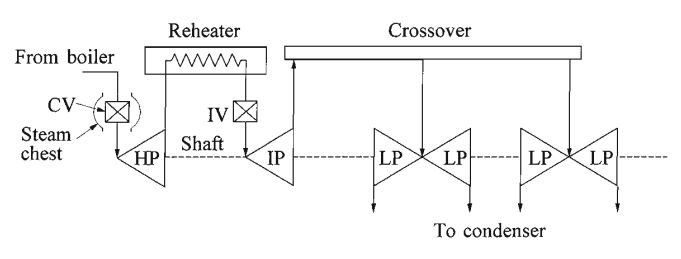
\includegraphics[scale=0.6]{./figures/A03_turbine_configuration}
	\caption{Execution of the main function creates \texttt{Env}, \texttt{Agent}, and \texttt{Demand} objects and passes them to a \texttt{ddpg\_train} function call}
	\label{fig:software_implementation}
\end{figure}